\documentclass{csse4400}

% \teachermodetrue

\usepackage{float}

\usepackage{languages}

\title{Empty Practical}
\author{Evan Hughes \& Brae Webb}

\date{\week{0}}
\begin{document}

\maketitle

\begin{figure}[h]
  \href{https://www.oreilly.com/library/view/designing-data-intensive-applications/9781491903063/ch02.html}{
    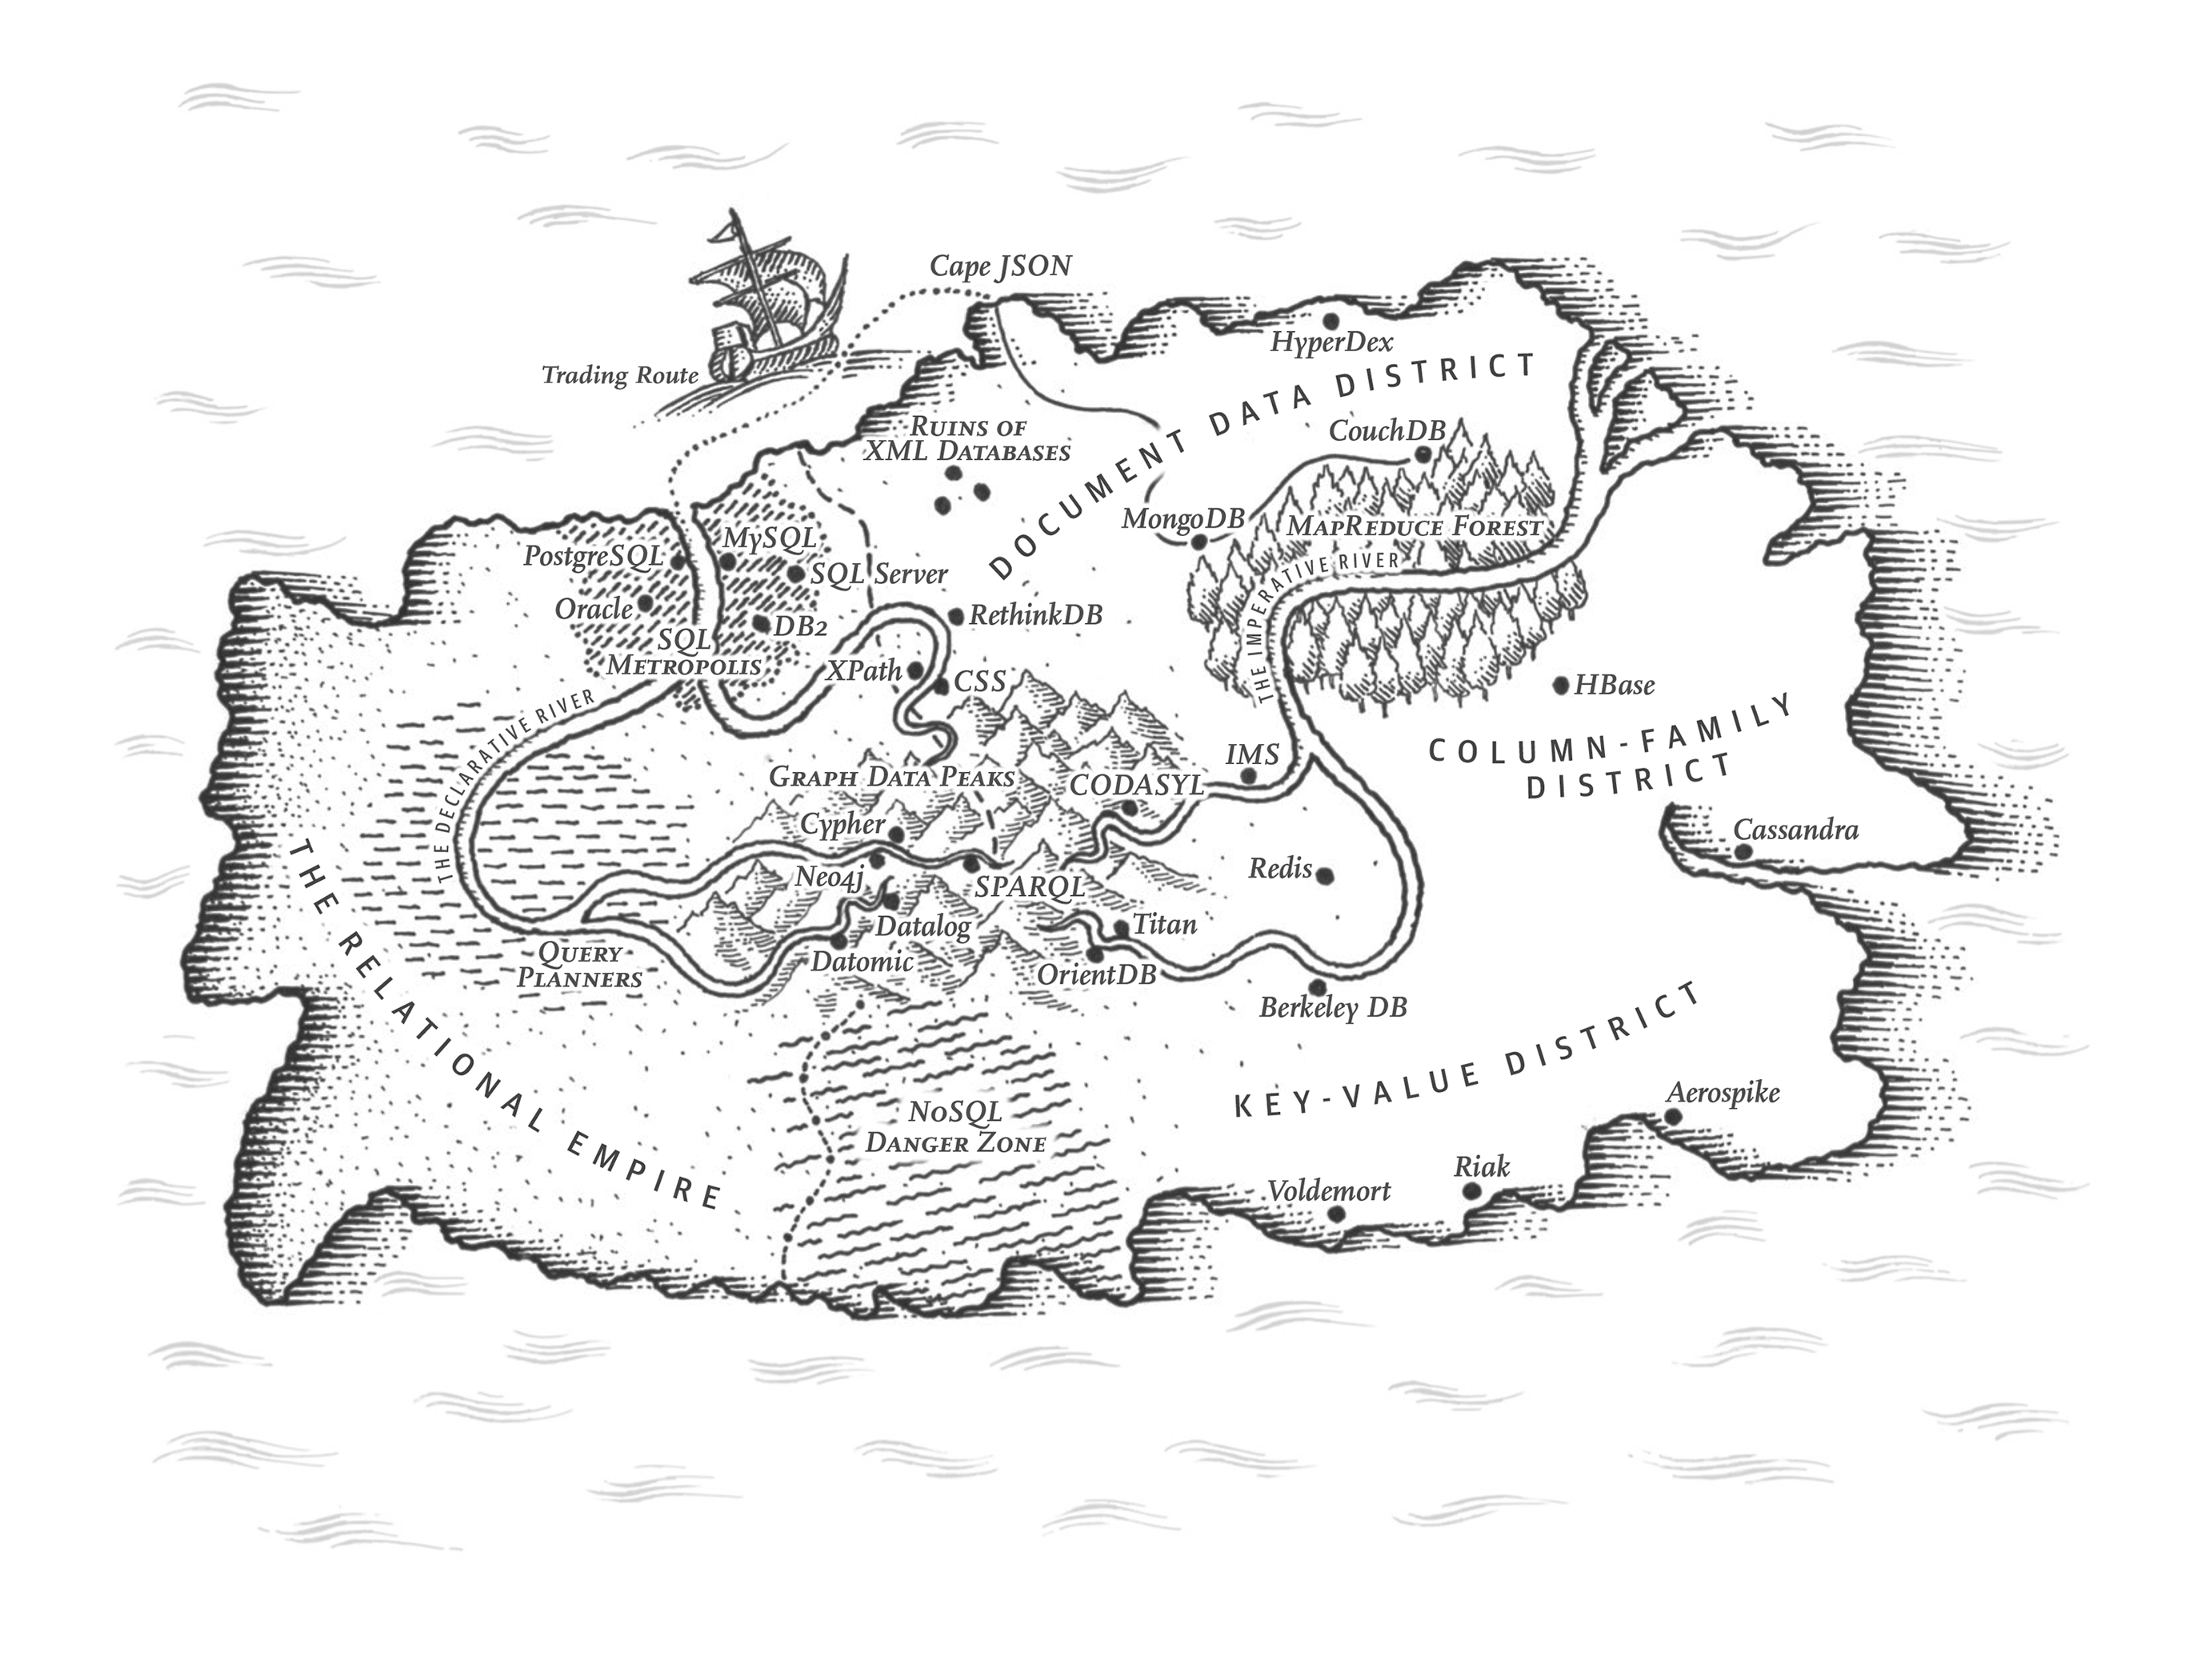
\includegraphics[width=\textwidth]{images/databases}
  }
\caption{A map of data storage techniques from Designing Data-Intensive Applications \cite{data-intensive}.}
\end{figure}

\section{This Week}
This week our goal is to:
\begin{itemize}
  \item fill in content here.
\end{itemize}

\section{Databases and Data Models}
stuff here.

\teacher{
  Knowledge for teaching.\\

  is here
}


\bibliographystyle{ieeetr}
\bibliography{books,ours}

\end{document}